\begin{figure}[tbp]
\begin{center}
\includegraphics[width=0.4\textwidth]{compare_bias_rsdsub_z1z2.eps}
\end{center}
\vspace{-0.7cm}
\caption{The bias $b=P_{\delta_\mathrm{nlRSD},\delta}/P_{\delta}$ 
of redshift space distorted(RSD) field after linear RSD substraction.
Dark lines indicate the $k_c$ cutoff---modes above them are assumed to be lost in noise.}
\label{fig:bias}
\end{figure}
The redshift space distortion(RSD) refers to the misjudgement on comoving distance 
resulting from peculiar velocity of objects. 
In this section we add the RSD effect to our original fields and 
present the cross correlation result in Fig.\ref{fig:r}. 
The influence is quite interesting. 

First, there is an improvement on tidal reconstruction results, 
%over all scales, 
which increases the cross correlation by 0.1 for nearly all $\ell$ demonstrated. 
Second, for noise substracted fields, the correlation on intermediate scales start to emerge.  

All these unexpected improvements can be attributed to the fortunate fact 
that RSD is in identical direction with foregrounds. 
The different behaviors are due to linear and non-linear RSD. 

Linearly RSD will induce an additional contraction in $z$ direction 
which increases with $z$.  
$\delta^\mathrm{RSD}(\bm{k})=(1+f\mu^2)\delta(\bm{k})$ 
with $\mu=k_\parallel/k$. 
If we divide the observed density contrast with $1+f\mu^2$, 
we can see how much non-linear effect presents. 
we show the bias between linearly substracted RSD field 
and real space field  
%$b=P_{\delta_\mathrm{nlRSD},\delta}/P_{\delta}$  
in Fig.\ref{fig:bias}. 
Dark lines indicate the small scale cut off. 
%Modes above $k_c$ are considered lost.
As we can see, 
for $z=2$, the modes we use are generally 
within linear RSD regions; 
for $z=1$, linear RSD still dominates, yet there are considerable non-linear RSD for large $k_\parallel$.  

The positive effect on tidal reconstruction is mainly caused by linear RSD
---that's why it is stronger on $z=2$ than $z=1$. 
The additional contraction $1+f\mu^2$ 
assigns more weights to larger $k_z$ modes, 
and give a preference on $\gamma_x,\gamma_y,\gamma_z$ in Eq.\ref{eq:gamma}.  
This happen to be consistent with the improvements we suggest in Section 
\ref{ssec:improve}, 
which reduces the weights of foreground contaminated modes, 
and increases the dependence on three shear estimators 
that are relatively clean. 
Therefore, the recovering results will better assemble original fields. 

For noise substracted fields, the higher cross correlations on large scales 
are caused by non-linear RSD. 
The contraction from linear RSD is corrected in Eq.\ref{eq:wienerv} 
by dividing the bias term. 
However, the non-linear RSD will induce extra noises that can not be 
directly suppressed by bias, and will lead to reduced weights in Wiener filter 
for small scale structure. 
Consider previously the null correlation is due to reduced weights on large scales due to foreground contamination. 
Now the small scale distortions somewhat rebalance the weights, 
which results to the appearance of a little correlation on smaller $\ell$. 
This effect is mainly seen on $z=1$ with stronger non-linear RSD.

In all, the RSD seems to be a blessing rather than a problem in our case. 
It also reveals the great potential of our reconstruction 
if applying more precise noise-related filter.  
And this is not the only advantage RSD brings. 
In reality, the inhancement in large $k_z$ will increase the S/N, 
and therefore raise the cut off scale $k_c$, which enables better tidal reconstruction results. 
